\chapter{Jade e Jason}

\section{Jade}

\subsection{FIPA}

\dfn{FIPA}{
  Consorzio per la standardizzazione di sistemi ad agenti. Il suo obiettivo era quello di promuovere tecnologie interoperabili: sistemi di agenti intelligenti che lavorano insieme.
}

\qs{}{Cosa rientrà nelle competenze di FIPA?}

\begin{itemize}
  \item Gestione del ciclo di vita di un agente. 
  \item Come trasportare un messaggio. 
  \item La struttura di un messaggio. 
  \item Protocolli di interazione tra agenti. 
  \item Ontologie e sicurezza.
\end{itemize}

\nt{Gli agenti sono al di fuori degli obiettivi di FIPA.}

\paragraph{Caratteristiche che vengono assunte per gli agenti:}

\begin{itemize}
  \item Autonomi. 
  \item Reattivi. 
  \item Proattivi. 
  \item Goal-driven. 
  \item Sociali. 
  \item Adattivi. 
  \item Cognitivi.
\end{itemize}

\begin{figure}[!h]
    \centering
    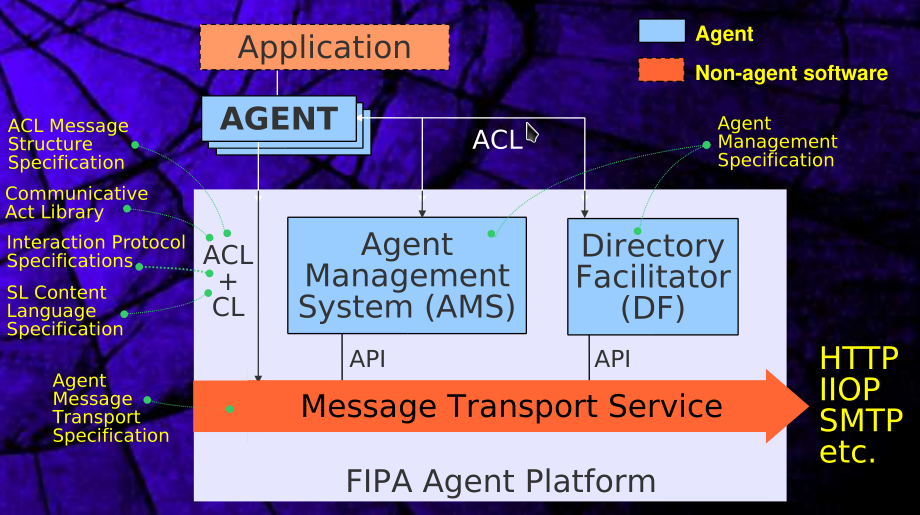
\includegraphics[scale=0.35]{05/FIPA.png}
  \caption{Piattaforma FIPA per agenti.}
\end{figure}

\cor{Agent Management}{
  Gli agenti hanno una descrizione di sé stessi e dei servizi che vengono offerti. L'Agent Management sistem è a sua volta un agente con cui si interagisce con scambi di messaggi. In jade si può accedere così oppure accedere direttamente agli oggetti Java.
}

\begin{figure}[!h]
    \centering
    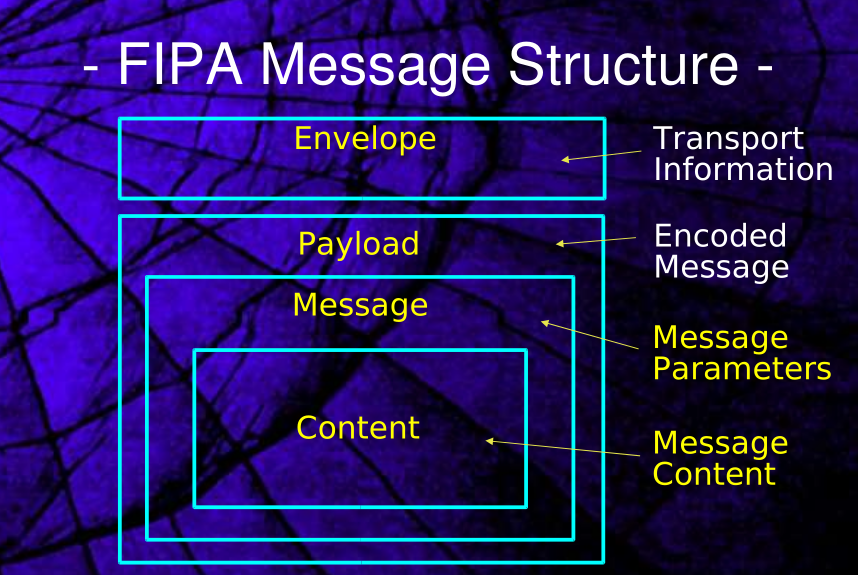
\includegraphics[scale=0.35]{05/messaggi.png}
  \caption{Specifica per i messaggi.}
\end{figure}

\subsection{Introduzione a JADE}

\qs{}{Che cos'è JADE?}

\paragraph{Risposta:} JADE è la piattaforma, all'interno del consorzio FIPA, che implementa lo standard sopra citato. Si presenta come codice Java puro. Offre una serie di librerie per agenti e un runtime envinronment per gli agenti creati. L'obiettivo è quello di "nascondere" FIPA al programmatore. 

\begin{figure}[!h]
    \centering
    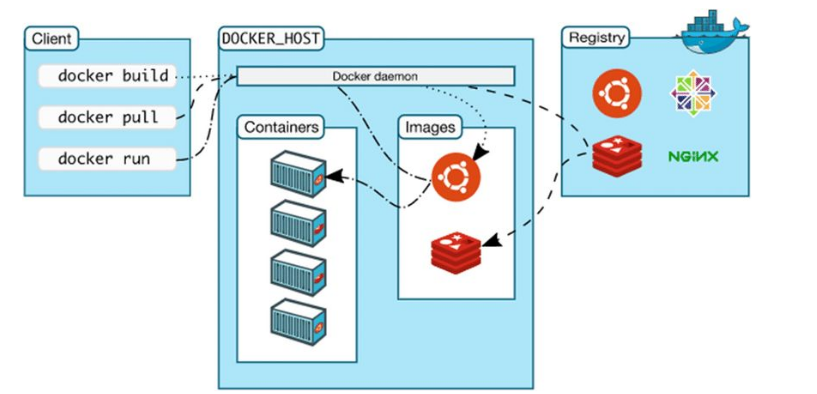
\includegraphics[scale=0.45]{05/arch.png}
  \caption{Modello architetturale di JADE.}
\end{figure}

\paragraph{Caratteristiche importanti:}

\begin{itemize}
  \item \fancyglitter{HalloWorld Agent:}
    \begin{itemize}
      \item Un tipo di agente è creato estendendo \texttt{jade.core.Agent} e ridefinendo il metodo \texttt{setup()}. 
      \item Ogni agente è identificato da un AID (nome univoco e qualche indirizzo).
      \item A ogni agente è assegnato uno e un solo thread (per evitare deadlock).
    \end{itemize}
  \item \fancyglitter{Local names, GUID and addresses:}
    \begin{itemize}
      \item Il nome completo di un agente deve essere globalmente unico. 
      \item In una singola piattaforma JADE ci si riferisce agli agenti solamente mediante il loro nome. 
      \item È possibile creare AID. 
      \item Si possono passare argomenti agli agenti.
    \end{itemize}
  \item \fancyglitter{Terminazione:}
    \begin{itemize}
      \item Un agente termina quando è chiamato il metodo \texttt{doDelete()}. Questo metodo non cancella all'istante, ma segnala che l'agente deve essere eliminato (solo dopo aver completato la \texttt{setup()}. 
      \item Nella terminazione è chiamato il metodo \texttt{takeDown()} per fare operazioni di clean-up.
    \end{itemize}
\end{itemize}

\dfn{Classe Behaviour}{
Il lavoro si un agente è eseguito dalle sue "behaviours". Per far sì che un agente esegua un task è sufficiente definire una behaviour e aggiungerla all'agente. 
}

\paragraph{Ogni behaviour deve implementare:}

\begin{itemize}
  \item \texttt{void action():} cosa la behaviour fa. 
  \item \texttt{boolean done():} quando la behaviour finisce.
\end{itemize}

\nt{Un agente può eseguire più behaviours in parallelo, il loro scheduling è cooperativo e tutti avvengono nello stesso thread java.}

\begin{figure}[!h]
    \centering
    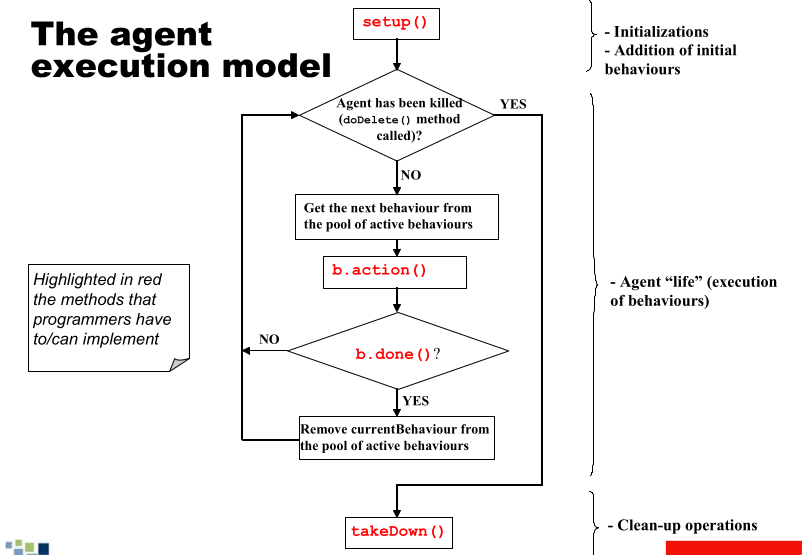
\includegraphics[scale=0.5]{05/exec.png}
  \caption{Modello di esecuzione di un agente.}
\end{figure}

\paragraph{Tipi di behaviour:}

\begin{itemize}
  \item \fancyglitter{One shot:}
    \begin{itemize}
      \item La loro \texttt{action()} viene eseguita solo una volta. 
      \item \texttt{done()} restituisce sempre true (non si deve reimplementare).
    \end{itemize}
  \item \fancyglitter{Cyclic:}
    \begin{itemize}
      \item Non si completano mai, \texttt{action()} effettua sempre le stesse operazioni. 
      \item \texttt{done()} restituisce sempre false (non si deve reimplementare).
    \end{itemize}
  \item \fancyglitter{Complex:}
    \begin{itemize}
      \item Hanno uno stato (e.g. DFA) e a seconda di esso svolgono operazioni differenti. 
      \item Completano quando una data condizione diventa vera.
    \end{itemize}
\end{itemize}







\section{Jason}
